\chapter{Projeto - Parte 1} \label{ch:projeto-parte1}

Esta parte do projeto incidiu principalmente sobre desenvolvimento de uma biblioteca, em Java, para providenciar abstrações dos subsistemas que representam conceito gerais de Inteligência Artificial (e.g., agente, ambiente) e outros conceitos relacionados (e.g., máquina de estados).

Para tal, foi necessário definir uma arquitetura de software que permitisse a implementação dos diferentes subsistemas de forma independente e modular, seguindo as diretrizes (i.e., métricas (ver secção~~\ref{subsec:metricas}) e princípios (ver secção~\ref{subsec:principios})) que garantem a qualidade da arquitetura.

Associado à elaboração da arquitetura de software, foi necessário definir um processo de desenvolvimento de software (ver secção~\ref{sec:processo-de-desenvolvimento-de-software}) que permitisse a implementação dos diferentes subsistemas de forma progressiva, através de diferentes níveis de abstracção (i.e., modelo, arquitetura e implementação).

A implementação da biblioteca foi feita com base na consulta e compressão de diagramas UML e de sequência de forma a garantir a correta implementação dos diferentes subsistemas e a sua interação.


\section{Arquitetura de software}\label{sec:arquitetura-de-software}

A arquitetura de software aborda a complexidade inerente ao desenvolvimento de software por meio de uma série de vertentes que estão interligadas.

\subsection{Métricas}\label{subsec:metricas}

As métricas são medidas de quantificação da arquitectura de um software indicadoras da qualidade dessa arquitectura;

O acomplamento é uma métrica inter-modular que mede o grau de interdependência entre os módulos de um sistema. Pode ser medido através da:
\begin{itemize}
    \item \textbf{Direção}: Unidirecional vs Bidirecional (uni representa menos acoplamento);
    \item \textbf{Visibilidade}: Quando menor for a visibilidade de um módulo, menor é o seu acoplamento;
    \item \textbf{Ordem}: (de menos acoplamento para mais) Herança $\rightarrow$ Composição $\rightarrow$ Agregação $\rightarrow$ Associação $\rightarrow$ Dependência.
\end{itemize}

A coesão é uma métrica intra-modular que determina o nível de coerência funcional de um subsistema/módulo, seja pela sua organização (i.e., cada modulo está organizado por conteúdo) ou pela sua funcionalidade (e.g., \ti{single responsibility principle} - cada modulo tem uma única responsabilidade).

\subsection{Princípios}\label{subsec:principios}

Os princípios no contexto da arquitectura de software são um conjunto de convenções que orientam a sua definição, garantindo a qualidade de produção da mesma. Alguns exemplos são:
\begin{itemize}
    \item \textbf{Abstração}: Define a forma como os componentes de um sistema são representados, permitindo a ocultação de detalhes de implementação;
    \item \textbf{Modularização}: Ao qual está associado a decomposição (e.g, divisão do sistema em sub-módulos) e o encapsulamento (i.e., ocultação de detalhes de implementação e/ou manutenção de estado privado e interno);
    \item \textbf{Factorização}: Onde a arquitectura é dividida em camadas, cada uma com um conjunto de responsabilidades bem definidas. Pode ser estrutural (e.g, Herança) e Funcional (e.g, Delegação);
\end{itemize}


\section{Processo de Desenvolvimento de Software}\label{sec:processo-de-desenvolvimento-de-software}

O processo de desenvolvimento de software consiste na
criação da organização de um sistema de forma
progressiva, através de diferentes níveis de abstracção:

\begin{itemize}
    \item \textbf{Modelo (Conceptual)}: Representação abstrata do sistema, que define o que o sistema deve fazer, sem especificar como;
    \item \textbf{Arquitetura (Modelo Concreto)}: Representação concreta do sistema, que define como o sistema deve ser implementado;
    \item \textbf{Implementação}: Código fonte que implementa o sistema definindo como o sistema deve ser executado.
\end{itemize}

Consiste num processo iterativo, em que as diferentes actividades de desenvolvimento são alternadas ao longo do tempo em função do conhecimento e do nível de detalhe
envolvido. Essa alternância poderá ser circular (i.e., implementação $\rightarrow$ arquitectura $\rightarrow$ modelo $\rightarrow$ implementação).

\subsection{Tipos de Implementação}\label{subsec:tipos-de-implementacao}

\begin{table}[H]
    \centering
    \caption{Tipos de Implementação}
    \label{tab:tipos-de-implementacao}
    \begin{tabular}{|l|l|p{8cm}|}
        \hline
        \textbf{Tipo}  & \textbf{Modelo Associado} & \textbf{Designação}                                                                                        \\ \hline
        Estrutural     & \ti{UML}                  & Define a estrutura de um sistema, ou seja, a forma como os componentes se relacionam entre si.             \\ \hline
        Comportamental & \ti{Sequence Diagram}     & Define o comportamento de um sistema, ou seja, a forma como os componentes interagem e comunicam entre si. \\ \hline
    \end{tabular}
\end{table}

Mais detalhadamente, os diagramas de sequência ou atividade representam o fluxo de controlo de um sistema, ou seja, a sequência de atividades que um sistema executa e a sua ordem. Definem-se como modelos de interação com uma organização bidirecional (i.e., horizontal $\rightarrow$ tempo e vertical $\rightarrow$ estrutura) e são compostos por diferentes elementos de modelação (e.g., mensagens, operadores, linha de vida).

Já a linguagem de modelação unificada (UML) representa um modelo de comportamento com interação como perspetiva principal de modelação. Este tipo de modelação descreve a forma como as partes de um sistema interagem entre si e com o exterior para produzir o comportamento do sistema.


\section{Desenvolvimento do Jogo}\label{sec:desenvolvimento-do-jogo}

Tendo por base os conceitos anteriormente abordados, que consolidaram a aprendizagem inerente à implementação da biblioteca, foi desenvolvido um jogo que a utiliza.
No processo de desenvolvimento do jogo, foi definido um conjunto de componentes que providenciam implementações concretas dos conceitos mencionados, adaptados ao contexto específico do jogo:

\begin{itemize}
    \item \textbf{Personagem}: Representa o agente do jogo;
    \item \textbf{Ambiente}: Representa o ambiente onde a Personagem opera;
    \item \textbf{Máquina de Estados}: Representa a máquina de estados associada ao controlo da Personagem.
    Ver figura~~\ref{fig:projeto-parte1-maqest-personagem}.
\end{itemize}

\begin{figure}[H]
    \begin{center}
        \resizebox{100mm}{!}{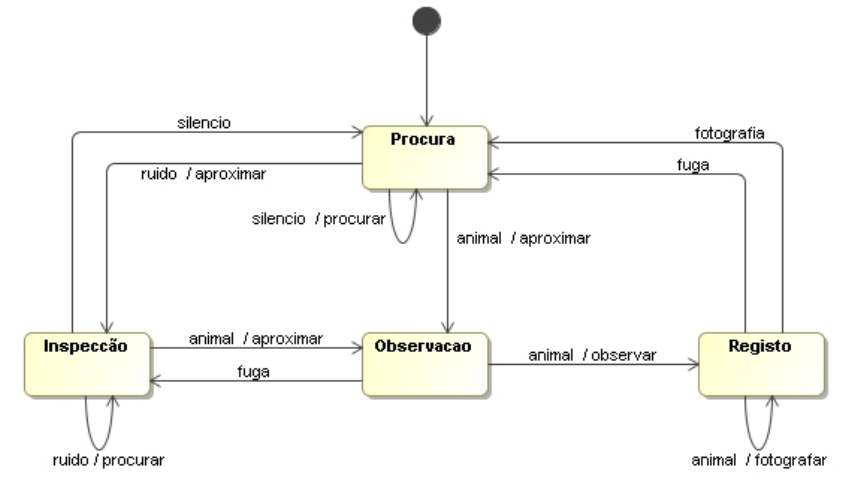
\includegraphics{../figures/projeto-parte1-maqest-personagem}}
    \end{center}
    \caption{Máquina de estados associada ao controlo da Personagem.}\label{fig:projeto-parte1-maqest-personagem}
\end{figure}

O jogo consiste num ambiente onde a personagem tem por objectivo registar a presença de animais através de fotografias.
O ambiente deste jogo, pode ser caracterizado (ver secção~\ref{sec:ambiente}) por ser:

\begin{itemize}
    \item \textbf{Virtual}: O ambiente é simulado e não existe fisicamente;
    \item \textbf{Totalmente Observável}: O agente tem acesso a uma descrição completa do ambiente e que lhe permite resolver o problema em questão sem necessitar de guardar estado interno;
    \item \textbf{De agente único}: Apenas existe um agente a atuar, neste caso, uma Personagem;
    \item \textbf{Determinístico}: O estado seguinte é unicamente determinado pelo estado actual e pela acção do agente;
    \item \textbf{Sequencial}: Pois existe uma linha de acontecimentos que se sucedem (e.g., não é possível inspeccionar, registar ou observar algo sem ser feita primeiro uma procura);
    \item \textbf{Estático}: Não se altera enquanto o agente está a tomar uma decisão;
    \item \textbf{Discreto}: O número de estados possíveis é finito.
\end{itemize}

Foi criada uma aplicação~\ref{fig:projeto-parte1-jogo} de \textif{cli} (i.e., command-line interface) em Java, que possibilita a interação com o jogador por meio de comandos em texto.
Tendo em conta que a interface gráfica não era o foco desta parte do projeto, foi emulada através de texto descritivo.

\begin{figure}[H]
    \begin{center}
        \resizebox{100mm}{!}{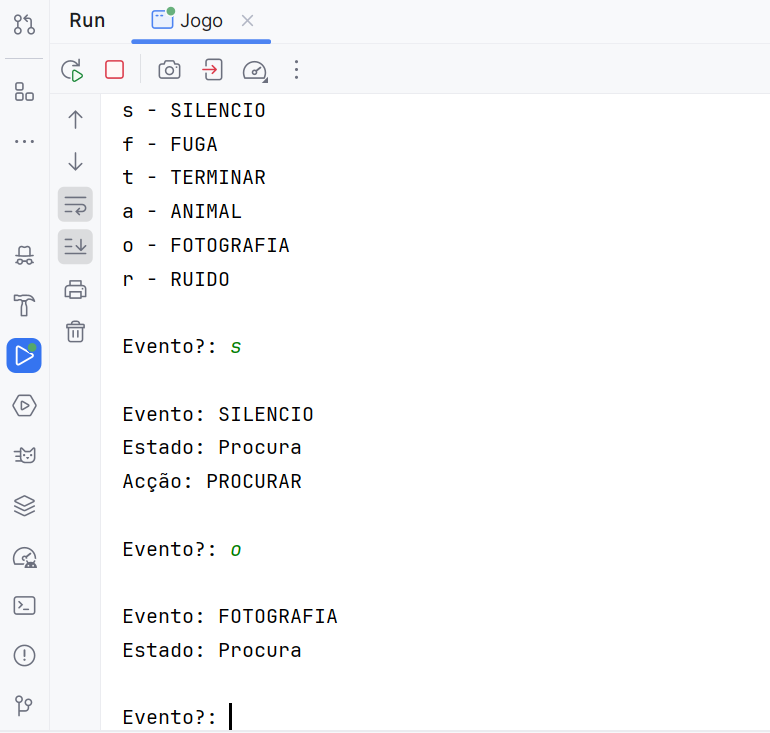
\includegraphics{../figures/projeto-parte1-jogo}}
    \end{center}
    \caption{Utilização da aplicação do jogo.}\label{fig:projeto-parte1-jogo}
\end{figure}

\section{Estrutura do Projeto}\label{sec:estrutura-do-projeto}

No processo de desenvolvimento de software associado a este projeto, foi definida a seguinte estrutura em módulos e que está presente na pasta \ti{iasa\_jogo/src}:

\begin{itemize}
    \item \textit{agente}: Integra classes e interfaces que definem o Agente e os seus componentes (e.g., módulo de controlo);
    \item \textit{ambiente}: Agrega interfaces que representam o Ambiente e os seus componentes (e.g., comandos, eventos);
    \item \textit{maqest}: Contém classes que definem o conceito de Máquina de Estados e os seus componentes (e.g., estados, transições);
    \item \textit{jogo}: Agrega os detalhes da implementação do jogo, onde são integrados os módulos anteriores e definidas implementações concretas dos mesmos, adequadas ao contexto a que o jogo se insere.
\end{itemize}
